% EBP course: session 3
% Thomas Klee
% 30 Jan 2019

% Preamble
\documentclass{beamer}
\usetheme{Singapore}
\usefonttheme[onlysmall]{structurebold}
\setbeamertemplate{footline}[frame number]
\setbeamerfont{title}{shape=\itshape,family=\rmfamily}
\usepackage{graphicx}
\usepackage[english]{babel}
\usepackage[utf8x]{inputenc}
\usepackage{amsfonts, amsmath, amsthm, amssymb} % for math fonts, symbols and environments
\usepackage{xcolor}
\usepackage{booktabs}
\usepackage{ctable} % for command-driven tables
\usepackage{wasysym} 
\usepackage[natbibapa]{apacite}

% activate following line for custom appearance
% \usepackage{beamerthemesplit} 

\mode<presentation>

% information for title slide
\title{Evaluating Intervention Evidence}
\subtitle{}
\author{Evidence-Based Practice in Speech-Language Therapy \\ (SHSC 2033)}
\institute{Session 3}
\date{Thomas Klee \& Elizabeth Barrett}
\titlegraphic{
\includegraphics[width=6cm]{images/logo_CE_C.jpg}} % HKU logo

\begin{document}

% create title slide with information above
\begin{frame}
	\titlepage
\end{frame}

% 
\begin{frame}{Outline}
	\begin{enumerate}
	\item Hierarchy of evidence
	\item Randomised controlled trials (RCTs)
	\item Reporting standards
	\item Critically appraising evidence
	\item Group discussion
	\end {enumerate}
\end{frame}

\section*{Hierarchy of Evidence}

%
\begin{frame}
\center{\Huge{\textcolor{darkgray}{Hierarchy of Evidence}}}
\end{frame}

% 
\begin{frame}{Hierarchy of evidence}
	\begin{itemize}
	\item Searching for evidence can turn up anything from well-designed research studies to expert opinions to personal opinions.
	\item Various schemes have been designed to rank the scientific value of different kinds of evidence.
	\item Consider the strength of evidence.
	\end {itemize}
\end{frame}

% 
\begin{frame}{Simple hierarchy of intervention evidence\footnote{\tiny{\citet[p. 18]{Greenhalgh2010}}}}
	\begin{center}
	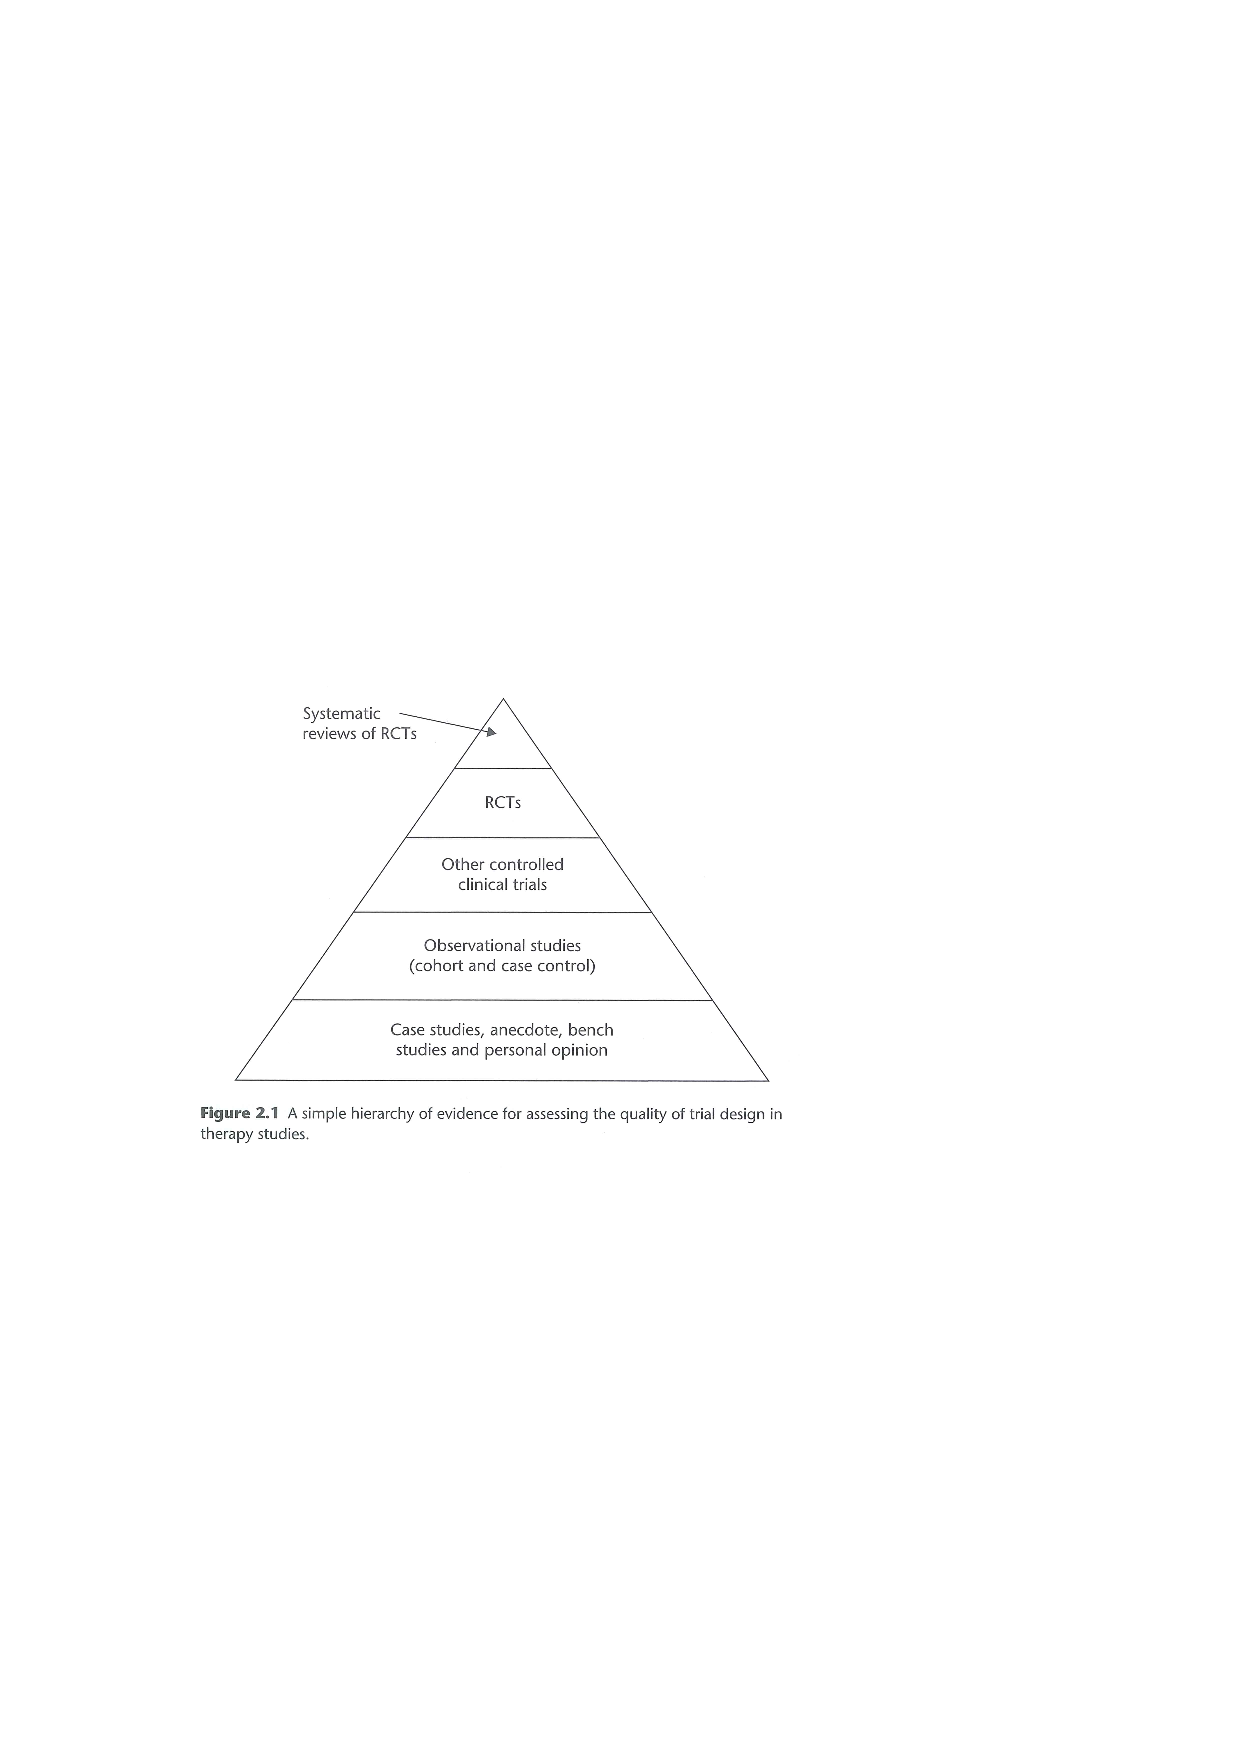
\includegraphics[width=.9\textwidth]{images/evidence_hierarchy_greenhalgh_4th.pdf}
	\end{center}
\end{frame}

% 
\begin{frame}{CEBM's levels of evidence for intervention studies\footnote{\scriptsize{Oxford Centre for Evidence-Based Medicine, 2009}}}
	\begin{itemize}
	\item[1a] Systematic reviews (SR) \& meta-analyses (with homogeneity) of RCTs
	\item[1b] Individual RCT (with narrow confidence interval)  
	\item[2a] SR (with homogeneity) of cohort studies
	\item[2b] Individual cohort study (including low quality RCT)
	\item[3a] SR (with homogeneity) of case-control studies
	\item[3b] Individual case-control studies
	\item[4] Case-series (and poor quality cohort and case-control studies)
	\item[5] Expert opinion without explicit critical appraisal; bench research
	\end{itemize}
\end{frame}

% 
\begin{frame}{Evidence hierarchies for other study types}
For evidence hierarchies relevant to studies related to prognosis, diagnosis, and economic and decision analyses, see the CEBM's website: 
\url{http://www.cebm.net/index.aspx?o=1025}
\end{frame}

\section*{RCTs}

%
\begin{frame}
\center{\Huge{\textcolor{darkgray}{RCTs}}}
\end{frame}

%
\begin{frame}{How effective is this for improving my fitness level?}
\url{https://support.apple.com/en-hk/HT204517}
\end{frame}

% 
\begin{frame}{Randomised controlled trials (RCTs)\footnote{\scriptsize{With thanks to David Howard, Newcastle University, UK}}}
	\begin{itemize}
	\item Two (or more) treatment conditions are compared by randomly allocating participants to groups and controlling for known sources of \textbf{study bias}.
	\item Designed to investigate:
		\begin{itemize}
		\item Treatment vs. no-treatment (control group)
		\item Treatment 1 vs Treatment 2
		\item Several treatments 
		\end{itemize}
	\item Level 1b of the Oxford evidence hierarchy
	\end {itemize}
\end{frame}

% 
\begin{frame}{RCTs}
	\begin{itemize}
	\item Designed to establish the average efficacy of a treatment and learn about frequently occurring side-effects.
	\item Treatment effects may be small and therefore undetectable, except when studied systematically on a large sample.
	\item Treatment effects may vary between people, making inferences from single case studies unreliable.
	\end {itemize}
\end{frame}

% 
\begin{frame}{RCTs}
	\begin{itemize}
	\item Designed to control for change due to:
		\begin{itemize}
		\item Spontaneous recovery unrelated to treatment;
		\item Maturation, in the case of children;
		\item Other, unexpected things.
		\end{itemize}
	\end {itemize}
\end{frame}

% 
\begin{frame}{Essential features of RCTs}
	\begin{itemize}
	\item Study participants should be \textbf{randomly allocated} to treatment groups.
		\begin{itemize}
		\item Neither research staff nor participants should be able to influence who gets what treatment.
		\item This is controlled by \textbf{blinding}.
		\item This reduces bias by equalising other factors that have not been accounted for in the design of the study.
		\end{itemize}
	\item The population from which the sample is drawn should be clearly defined.
		\begin{itemize}
		\item Results only \textbf{generalise} to people from the same population, receiving the same treatment.
		\end{itemize}
	\end {itemize}
\end{frame}

% 
\begin{frame}{Essentials features of RCTs}
	\begin{itemize}
	\item The treatments should be clearly defined (e.g., ``manualized").
		\begin{itemize}
		\item This enables others to use the same treatment if it is effective.
		\item Sometimes available on a website; e.g. Lidcombe programme manual\footnote{\tiny{\url{https://sydney.edu.au/health-sciences/asrc/docs/lp_treatment_guide_2016.pdf}}}
		\end{itemize}
	\item The outcome measures should be clearly defined and relevant to the kinds of benefits anticipated.
		\begin{itemize}
		\item They should show what kind of benefit and the degree of benefit that can be expected from the intervention.
		\end {itemize}
	\end {itemize}
\end{frame}

% 
\begin{frame}{Blinding}
	\begin{itemize}
	\item An important study design feature to control bias.
	\item Single-blind trial
		\begin{itemize}
		\item Researcher knows the details of the treatment but the patient does not.
		\item Eliminates \textbf{placebo effects}, but \textbf{observer bias} is possible.
		\end{itemize}
	\item Double-blind trial
		\begin{itemize}
		\item Clinician, patient and assessor do not know which group the patient was assigned to.
		\end{itemize}
	\item Not always possible or practical, especially with behavioural interventions.
	\item \textbf{Blind assessors} are very important and usually possible.
	\end {itemize}
\end{frame}

% 
\begin{frame}{RCT data analysis}
	\begin{itemize}
	\item Patients are normally analysed within the group to which they were allocated, regardless of whether they experienced the intended intervention (\textbf{intention-to-treat analysis}).
	\item ``Intention-to-treat analyses are pragmatic in that they reflect real-world non-adherence to treatment.'' \footnote{\tiny{\url{http://hbiostat.org/doc/glossary.pdf}}}
	\item The analysis is focused on estimating the size of the difference in outcomes between intervention groups (effect size).
	\end {itemize}
\end{frame}

% 
\begin{frame}{Limitations of RCTs}
	\begin{itemize}
	\item Exposing patients to an intervention believed to be inferior to current treatment is sometimes considered unethical.
	\item On the other hand, failure to perform trials may result in harmful (or worthless) treatments being used.
	\item Once an intervention becomes widespread, it can prove impossible to recruit clinicians who are willing to \emph{experiment} with alternatives.
	\end{itemize}
\end{frame}

% 
\begin{frame}{Further limitations}
	\begin{itemize}
	\item RCTs are generally more costly and time consuming than other kinds of studies.
	\item Is the intervention well enough developed to permit evaluation?
	\item Is there preliminary evidence that the intervention is likely to be beneficial, from other sources of evidence?
	\item Is there an appreciation of the size of the treatment effect? (Needed to estimate sample size and justify expense of a trial.)
	\end{itemize}
\end{frame}

% 
\begin{frame}{Benefit of RCTs}
Well-designed and executed RCTs are the most rigorous way of determining whether a cause-effect relation exists between treatment and outcome and for assessing the cost-effectiveness of a treatment.
\end{frame}

\section*{Reporting Standards}

%
\begin{frame}
\center{\Huge{\textcolor{darkgray}{Reporting Standards}}}
\end{frame}

% 
\begin{frame}{Reporting standards}
	\begin{itemize}
	\item To promote transparent and complete reporting of RCTs
	\item CONSORT is evidence-based.
	\item The CONSORT 2010 statement
		\begin{itemize}
		\item For authors of RCTs
		\item 25-item checklist + flow diagram
		\item Chinese translation available\footnote{\scriptsize{http://www.consort-statement.org/downloads/translations}}
		\item \url{http://www.consort-statement.org}
		\end {itemize}
	\item The EQUATOR network
		\begin{itemize}
		\item One-stop website for reporting standards for most kinds of clinical studies, including \textbf{qualitative studies}
		\item \url{http://www.equator-network.org}
		\end{itemize}
	\end {itemize}
\end{frame}

\section*{Critical Appraisal}

%
\begin{frame}
\center{\Huge{\textcolor{darkgray}{Critical Appraisal}}}
\end{frame}

% 
\begin{frame}{Critically appraising evidence}
	\begin{itemize}
	\item Just because an RCT has been published doesn't guarantee that it was done well.
	\item Critical appraisal lets you judge for yourself about a study's quality and its value and relevance to your clinical practice.
	\end {itemize}
\end{frame}

% 
\begin{frame}{Critical appraisal checklists}
	\begin{itemize}
	\item For RCTs and many other kinds of clinical studies
	\item Dollaghan (2007) checklists
		\begin{itemize}
		\item Appendices A--E (may be photocopied; see p. 152)
		\item We'll use these in the group discussions in class.
		\end{itemize}
	\item Scottish Intercollegiate Guidelines Network (SIGN)
		\begin{itemize}
		\item \url{http://www.sign.ac.uk/checklists-and-notes.html}
		\end{itemize} 
	\item Oxford CEBM
		\begin{itemize}
		\item \url{http://www.cebm.net/index.aspx?o=1157}
		\end{itemize} 	
	\end{itemize}
\end{frame}

% \section*{Group Discussion}

% 
\begin{frame}{Group discussion}
	\begin{itemize}
	\item Break up into your assigned groups.
	\item Use CATE\footnote{\tiny{\citet[p. 153]{Dollaghan2007}}} to critically appraise the research articles you read for today.
	\item Document on the form \emph{where} you found information in the research article addressing each point.
	\item After the discussion, you may be asked to summarise several points on CATE.
	\end{itemize}
\end{frame}

%
\begin{frame}%[allowframebreaks] %[shrink=15] % to reduce font size of references
	\frametitle{References}
	\bibliographystyle{apacite}
	\small\bibliography{/Users/thomasklee/Documents/Bibtex/library}
\end{frame}

\end{document}